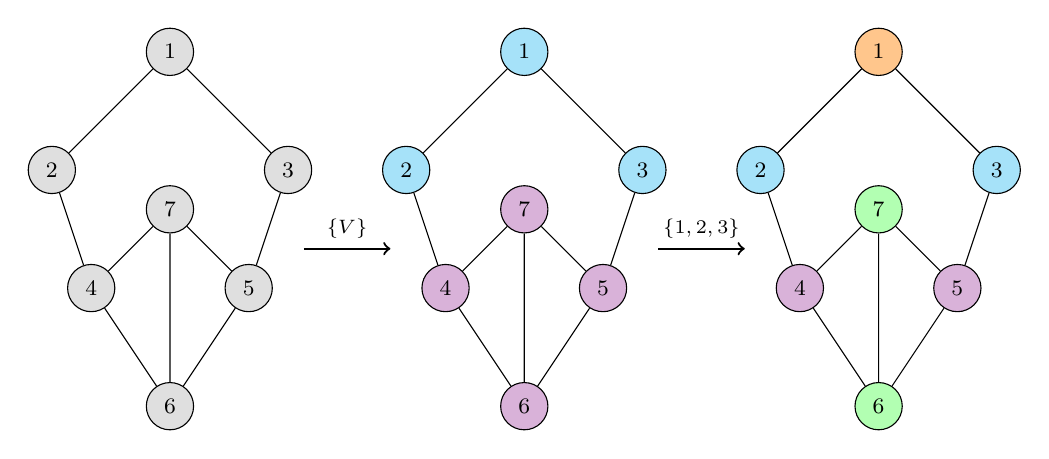
\begin{tikzpicture}
    \tikzset{v/.style={circle, draw, minimum size=6mm, inner sep=0pt, font=\footnotesize}}
    
    % ---- Panel 1: pi_0 (partition initiale) ----
    \begin{scope}
    \node[v, fill=gray!25] (a1) at (0,2.5) {1};
    \node[v, fill=gray!25] (a2) at (-1.5,1) {2};
    \node[v, fill=gray!25] (a3) at (1.5,1) {3};
    \node[v, fill=gray!25] (a4) at (-1,-0.5) {4};
    \node[v, fill=gray!25] (a5) at (1,-0.5) {5};
    \node[v, fill=gray!25] (a6) at (0,-2) {6};
    \node[v, fill=gray!25] (a7) at (0,0.5) {7};
    \draw (a1)--(a2) (a1)--(a3) (a2)--(a4) (a3)--(a5)
          (a4)--(a6) (a5)--(a6) (a4)--(a7) (a5)--(a7) (a6)--(a7);
    \end{scope}
    
    % ---- Panel 2: pi_1 (apres W=V) ----
    \begin{scope}[xshift=4.5cm]
    \node[v, fill=cyan!35] (b1) at (0,2.5) {1};
    \node[v, fill=cyan!35] (b2) at (-1.5,1) {2};
    \node[v, fill=cyan!35] (b3) at (1.5,1) {3};
    \node[v, fill=violet!30] (b4) at (-1,-0.5) {4};
    \node[v, fill=violet!30] (b5) at (1,-0.5) {5};
    \node[v, fill=violet!30] (b6) at (0,-2) {6};
    \node[v, fill=violet!30] (b7) at (0,0.5) {7};
    \draw (b1)--(b2) (b1)--(b3) (b2)--(b4) (b3)--(b5)
          (b4)--(b6) (b5)--(b6) (b4)--(b7) (b5)--(b7) (b6)--(b7);
    \end{scope}
    
    % ---- Panel 3: pi_2 = pi_final (apres W={1,2,3}) ----
    \begin{scope}[xshift=9cm]
    \node[v, fill=orange!45] (c1) at (0,2.5) {1};
    \node[v, fill=cyan!35] (c2) at (-1.5,1) {2};
    \node[v, fill=cyan!35] (c3) at (1.5,1) {3};
    \node[v, fill=violet!30] (c4) at (-1,-0.5) {4};
    \node[v, fill=violet!30] (c5) at (1,-0.5) {5};
    \node[v, fill=green!30] (c6) at (0,-2) {6};
    \node[v, fill=green!30] (c7) at (0,0.5) {7};
    \draw (c1)--(c2) (c1)--(c3) (c2)--(c4) (c3)--(c5)
          (c4)--(c6) (c5)--(c6) (c4)--(c7) (c5)--(c7) (c6)--(c7);
    \end{scope}
    
    % ---- Arrows between panels ----
    \draw[->, thick] (1.7,0) -- node[above, font=\scriptsize] {$\{V\}$} (2.8,0);
    \draw[->, thick] (6.2,0) -- node[above, font=\scriptsize] {$\{1,2,3\}$} (7.3,0);
    \end{tikzpicture}